\chapter{State of the Art}%
\label{chapter:State of the Art}

\begin{introduction}
This chapter will provide a comprehensive review of current \ac{5G} and Wi-Fi integration efforts, existing authentication mechanisms, and challenges in device identification. It will also explore recent developments and proposed solutions in the field, setting the context for our research.
\end{introduction}

\section{Why \acs{4G} needed improved security?}

From the point of view of authentication, a cellular network consists of three main components: User Equipment (UE), a Serving Network (SN), and a Home Network (HN).

The UE refers to devices like smartphones, tablets, or IoT devices equipped with a UICC  hosting at least a Universal Subscriber Identity Module (USIM) storing a cryptographic key that is shared with the subscriber’s home network. These devices connect to the network over radio signals. In 4G networks, these signals are based on technologies like LTE (Long-Term Evolution), utilizing frequency bands allocated for mobile communication.

The Serving Network (SN) includes network components that facilitate communication and provide services to the UE in a specific geographic area. Key elements of the SN are the eNodeB (Evolved Node B) and the MME (Mobility Management Entity).

\begin{itemize}
    \item{
        The eNodeB is a base station that manages the radio connection between the UE and the network. It handles tasks like scheduling radio resources, modulating and demodulating signals, and ensuring reliable data transmission over the air interface.
    }
    \item {
        The MME is a core network element responsible for managing signaling between the UE and the core network. It plays a key role in tasks such as authenticating the user, establishing bearers (data pathways), and ensuring mobility by managing handovers between eNodeBs as the UE moves.
    }
\end{itemize}

The Home Network (HN) refers to the network operated by the user's mobile service provider (e.g., MEO, Vodafone, or NOS). It stores subscriber information in a database called the Home Subscriber Server (HSS).

\begin{itemize}
    \item {
        The HSS is a critical component that contains user-specific data, such as subscription profiles, service entitlements, and cryptographic keys. These keys are used during the authentication process to verify that the user is authorized to access the network. The HSS communicates with the SN to authenticate the UE using protocols like Diameter over an IP-based system. This ensures secure and efficient exchange of authentication and session-related information.
    }
\end{itemize}

Communication between the SN and HN over the IP network is facilitated by core network protocols. The SN sends a request to the HSS containing the UE’s credentials (e.g., IMSI, International Mobile Subscriber Identity). The HSS uses its stored keys to generate authentication vectors, which are then sent back to the SN. The SN uses these vectors to authenticate the UE and establish a secure connection.

Together, these components form the Evolved Packet System (EPS)~\cite{cbl-comp-4g-5g-p3}, the architecture underlying 4G LTE networks. The EPS enables seamless connectivity and service delivery by integrating the radio access network (eNodeBs) with the core network components (e.g., MME and HSS). This design ensures that authentication, data management, and mobility are handled efficiently while providing high-speed, low-latency connections for the UE.

Prior generations to 4G, especially in Radio Access Networks (RANs), have faced significant security and privacy challenges. One major issue was the lack of network authentication in 2G, which allowed attackers to perform network spoofing using fake base stations. For example, a fake base station could advertise a stronger signal and lure User Equipment (UE) away from its legitimate network, enabling the attacker to send fraudulent text messages to the user.

Another issue was the lack of integrity protection for signaling messages, which left them vulnerable to spoofing and tampering. For instance, fake base stations could send unprotected Identity Request messages (a Non-Access Stratum [NAS] signaling message in LTE) to steal permanent UE identifiers, such as the IMSI.

Additionally, certain messages lacked confidentiality, resulting in privacy violations. For example, unencrypted paging messages could be intercepted to detect a user’s presence and track their precise location. 

To mitigate these vulnerabilities, the 3GPP introduced the Authentication and Key Agreement (AKA) protocol, which ensures entity authentication, message integrity, and message confidentiality. AKA employs a challenge-response mechanism based on a symmetric key shared between the subscriber and their home network. It also derives cryptographic keying materials to protect both signaling messages and user plane data, including communications over radio channels. This protocol significantly enhances security and privacy in mobile networks.

In 4G EPS-AKA, despite the enhancements brought by the 3GPP AKA protocol, two significant flaws remain. First, during the initial stage of the authentication process (the flow is shown in Figure \ref{fig:4g-authentication-flow}), the User Equipment (UE) must transmit its identity, specifically its IMSI, to the serving network. This identity is sent over the radio network without encryption, leaving it vulnerable to interception~\cite{cbl-comp-4g-5g-p3}. Although the use of a temporary identifier, such as the Globally Unique Temporary Identifier (GUTI), is intended to mitigate this risk, researchers have demonstrated that GUTI allocation is flawed in that the identifiers either do not change frequently enough~\cite{gt-freq} or are assigned in predictable patterns~\cite{gt-pred}.

Second, during the authentication decision, the home network may provide an Authentication Vector (AV), but this value is not directly included in the decision-making process, which is handled solely by the serving network~\cite{cbl-comp-4g-5g-p4}.

\begin{figure}[htbp]
    \centering
    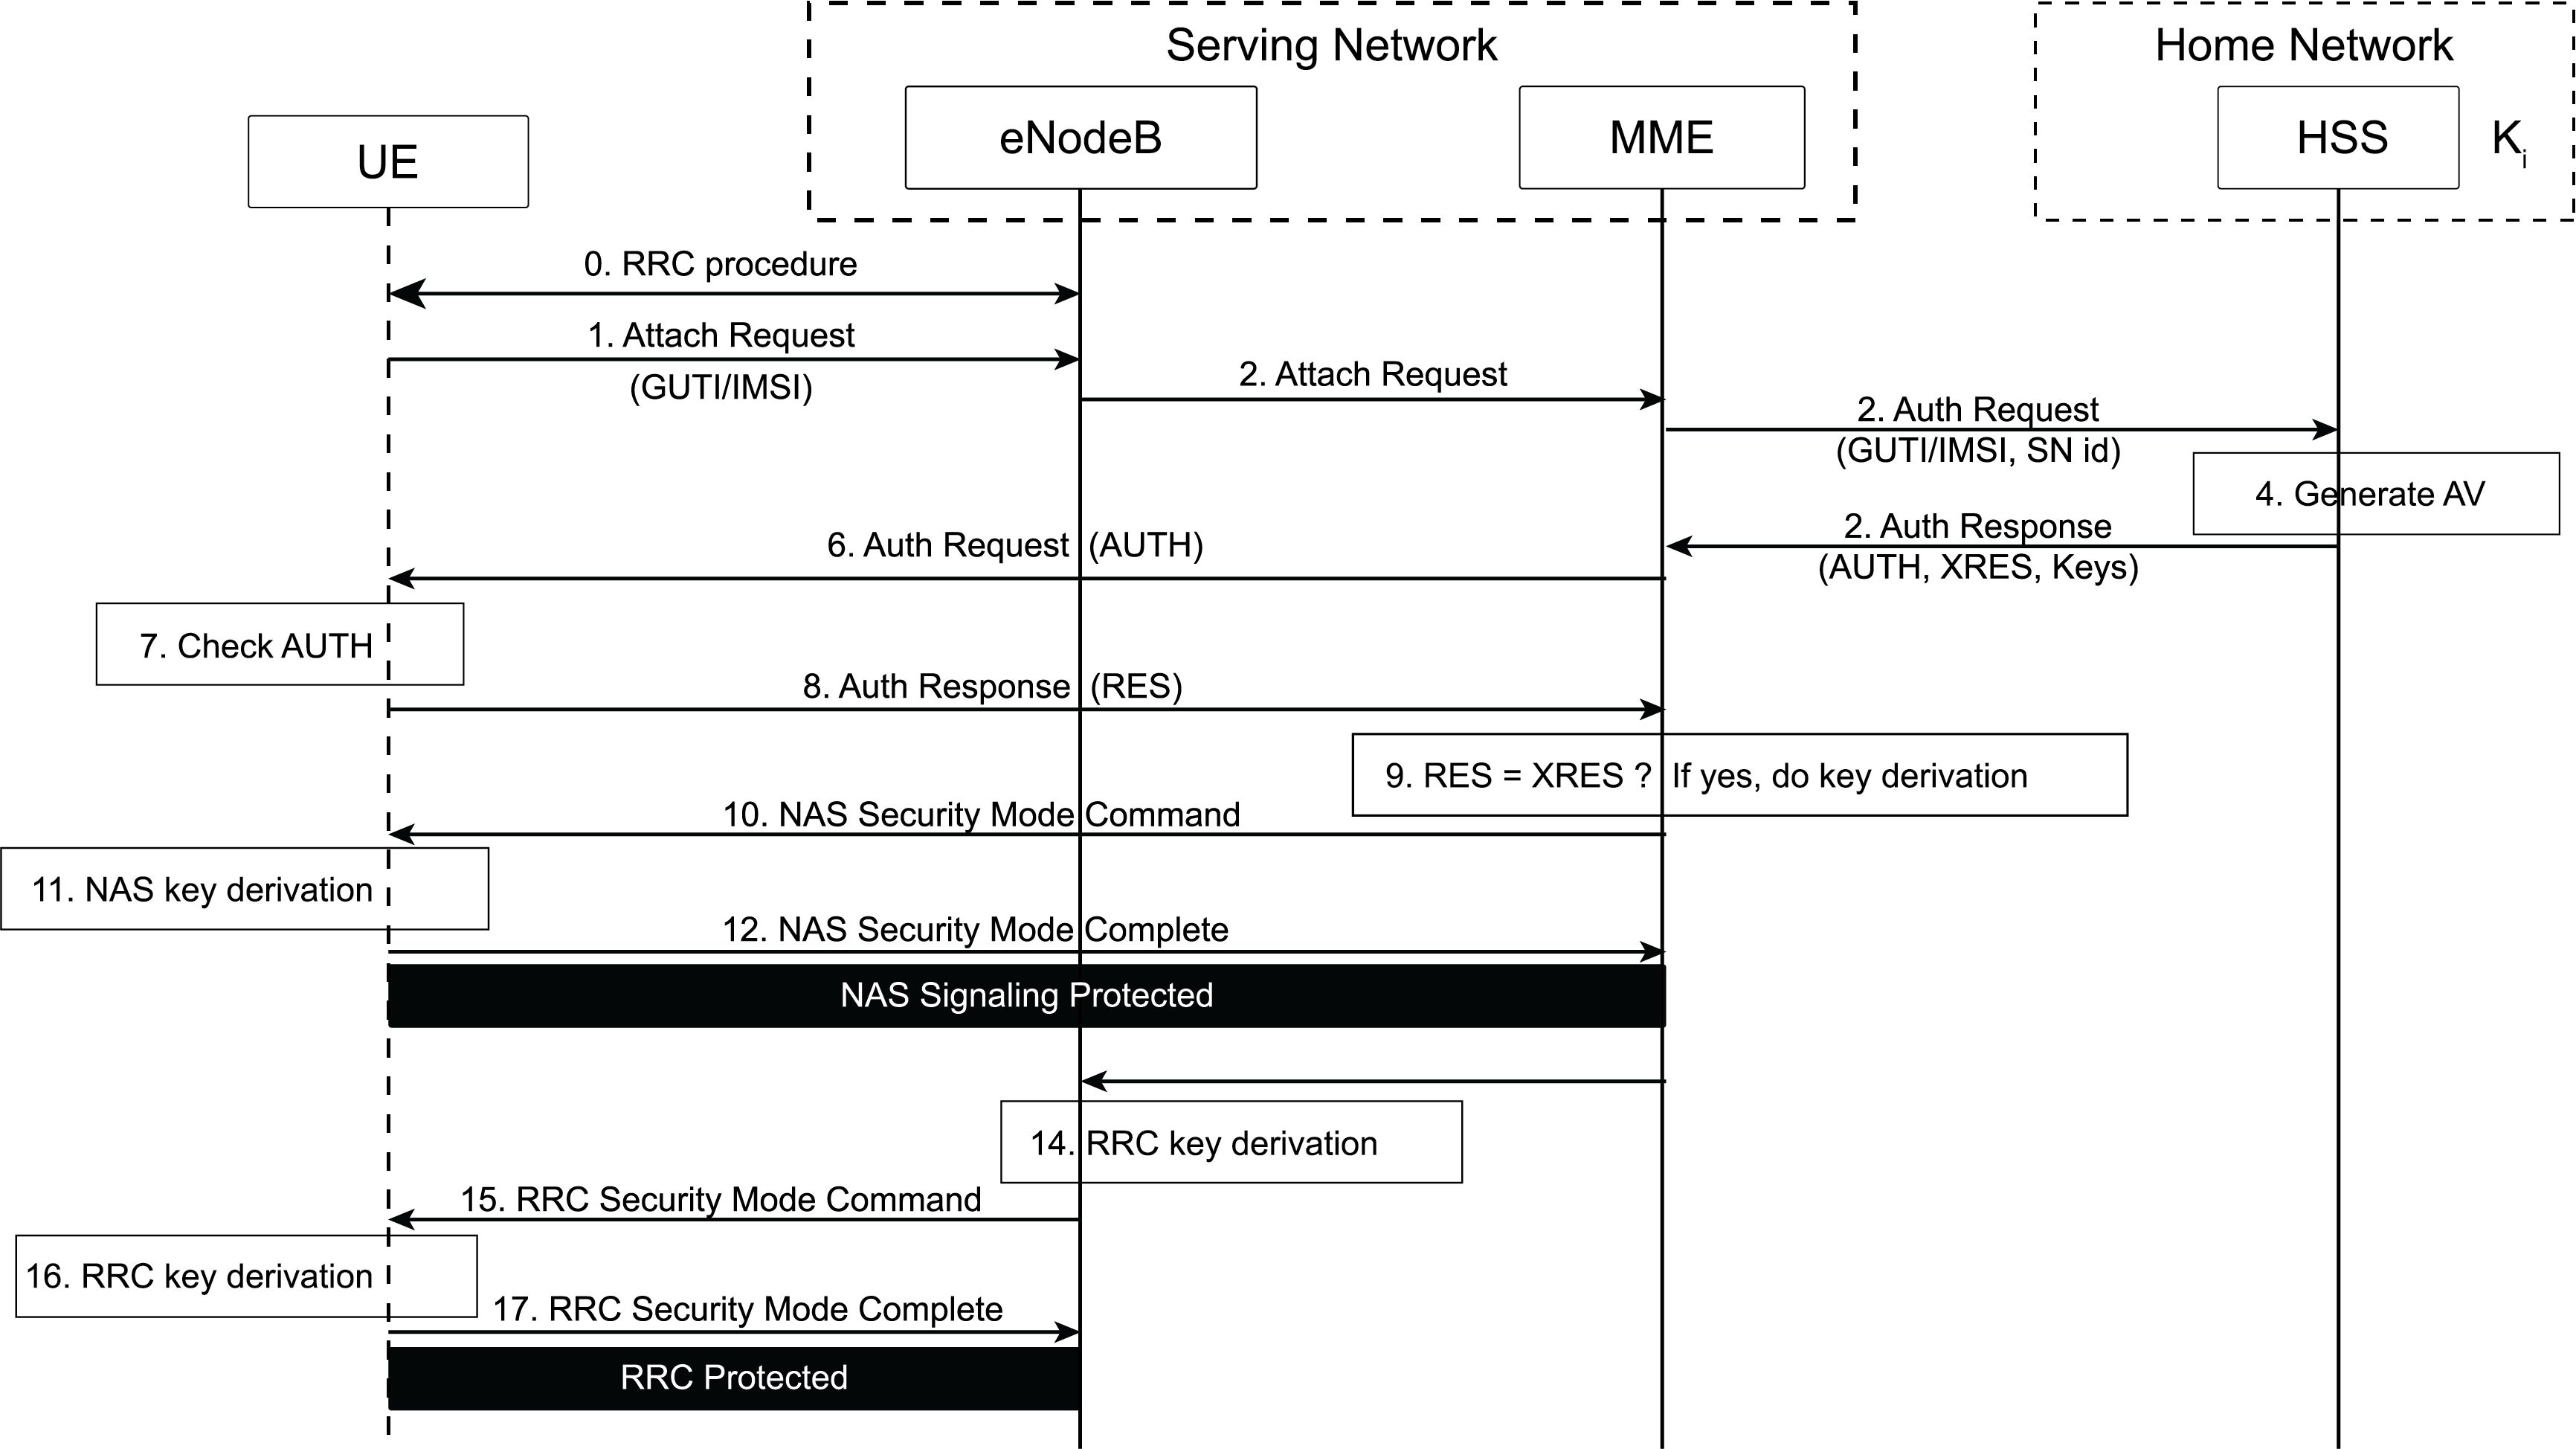
\includegraphics[width=0.8\textwidth]{figs/4g-authentication-flow.png}
    \caption{\ac{4G} Authentication Procedure}
    \label{fig:4g-authentication-flow}
\end{figure}

\section{\acs{5G} Architecture and Security Framework}

The 5G System architecture is designed to support advanced techniques such as Network Function Virtualization (NFV) and Software-Defined Networking (SDN). It separates Control Plane (CP) and User Plane (UP) functions, enabling independent scalability, evolution, and flexible deployments in centralized or distributed locations. The architecture uses modular function design to support efficient network slicing and defines procedures as reusable services to enhance flexibility. It minimizes dependencies between the Access Network (AN) and the Core Network (CN) by integrating different access types, including 3GPP and non-3GPP, through a converged core network.

The system includes a unified authentication framework, supports stateless Network Functions (NFs) by decoupling compute and storage resources, and enables capability exposure for network features. It allows concurrent access to local and centralized services and deploys UP functions near the Access Network to support low latency services and local data network access. Additionally, it supports roaming with both home-routed and local breakout traffic in visited networks, ensuring efficient and flexible operation.%cite 23.501 4.1

In 5G, the security framework is built around a new way of organizing the network, known as Service-Based Architecture (SBA). This setup introduces new entities and processes that focus on keeping the network secure, especially when it comes to authentication, which is the process of verifying users and devices.

% cite 23.501 6.2.X for each
\begin{itemize}
    \item{
        One of the key entities is the Security Anchor Function (SEAF), located in the serving network. Acrting as an intermediary during the authentication process. The SEAF receives authentication requests from a device (UE), but it relies on the home network to decide whether the authentication is valid or not. It can reject the authentication, but the final decision rests with the home network.
    }
    \item{
        The Authentication Server Function (AUSF) is the entity in the home network that actually decides whether the device should be allowed onto the network. The AUSF looks at the information provided by the device and checks it against the home network's security policies. It then works with other backend services to compute the necessary data and keys needed to authenticate the device, using secure methods like 5G-AKA or EAP-AKA’.
    }
    \item{
        The Unified Data Management (UDM) is in charge of managing the data involved in authentication. One of its key roles is managing the Authentication Credential Repository and Processing Function (ARPF), which selects the right authentication method based on the device's identity and the network's policies. It also helps generate the keys and data that the AUSF uses for authentication.
    }
    \item{
        Finally, the Subscription Identifier De-concealing Function (SIDF) helps protect the subscriber's permanent identity (called the SUPI). In 5G, this permanent identity, which could be something like a user’s IMSI, is always kept hidden and encrypted when sent over the air to prevent hackers from tracking it. The SIDF is the only part of the network that can decrypt the encrypted identity (called the SUCI) using a private key, ensuring that no one else can access the user’s personal details.
    }
\end{itemize}

At its core, this framework introduces a unified and flexible authentication system that seamlessly integrates both 3GPP (traditional cellular) and non-3GPP (such as Wi-Fi or cable) networks. This cross-network compatibility is crucial for enabling a wide range of access methods and supporting the growing ecosystem of connected devices.

Central to this framework is the Extensible Authentication Protocol (EAP), which facilitates secure communication between the User Equipment (UE) and the Authentication Server Function (AUSF). The Security Anchor Function (SEAF) acts as an intermediary, relaying authentication messages between the UE and AUSF. This setup supports various authentication methods, including 5G-AKA, EAP-AKA', and EAP-TLS, providing robust security for data exchange. For untrusted non-3GPP access, the Non-3GPP Interworking Function (N3IWF) comes into play, establishing a secure IPsec tunnel between the UE and the 5G core network, ensuring encrypted communication even over potentially insecure networks.%cite 23.501 6.2.x for NF

A key innovation in the 5G authentication framework is its ability to establish multiple security contexts during a single authentication process. This feature allows users to transition seamlessly between different network types without the need for re-authentication, significantly enhancing user experience and maintaining continuous secure access. Furthermore, the framework introduces improved subscriber privacy through the use of concealed subscriber identities (SUCI), protecting users from potential tracking or interception of their permanent identities (SUPI).%First part needs citation

\subsection{Comparing \acs{5G-AKA}, \ac{EAP-AKA'} and \ac{EAP-TLS}}

The 5G-AKA authentication process begins when the Security Anchor Function (SEAF) receives a request from the User Equipment (UE) seeking network access. The UE provides either a 5G-GUTI (Globally Unique Temporary Identifier) or a SUCI (Subscription Concealed Identifier) to begin the authentication. The AUSF (Authentication Server Function) first ensures that the requesting network is legitimate, then it sends an authentication request to the UDM/ARPF (Unified Data Management/Authentication Credential Repository and Processing Function). If the SUCI is provided, the SIDF (Subscription Identifier De-concealing Function) decrypts it to obtain the SUPI (Subscription Permanent Identifier), which is used to determine the authentication method.%cite 33.501 or 23.501

% add image of 5G-AKA flow

Next, the UDM/ARPF generates an authentication response containing tokens and keys. These are sent to the AUSF, which computes a hash (HXRES) and checks the expected response. The AUSF sends the authentication result, including the AUTH token and HXRES, to the SEAF, ensuring that the SUPI is not exposed to the SEAF, preserving privacy. The SEAF forwards the AUTH token to the UE, which then validates it using a secret key shared with the home network. If successful, the UE computes a RES token and sends it back to the SEAF. The SEAF forwards this to the AUSF, which validates the response.

Once the RES token is verified, the AUSF sends an anchor key to the SEAF. The SEAF derives an AMF key, which the AMF (Access and Mobility Management Function) uses to generate further keys for securing signaling messages between the UE and network elements. The UE, using its root key, can derive all necessary keys for secure communication with the network, ensuring mutual trust and security.

% add image of EAP-AKA' flow

An alternative authentication method in 5G is EAP-AKA', which provides mutual authentication between the UE and the network using a shared cryptographic key. Unlike 5G-AKA, EAP-AKA' uses EAP messages (Extensible Authentication Protocol) within NAS messages (Non-Access Stratum) between the UE and SEAF, and between the SEAF and AUSF. In EAP-AKA', the SEAF merely relays messages between the UE and the AUSF without making authentication decisions. In contrast, in 5G-AKA, the SEAF verifies the UE's authentication response and can act on failures. The KAUSF key in 5G-AKA is generated by the UDM/ARPF and sent to the AUSF, while in EAP-AKA', the AUSF derives this key from the EMSK (Extended Master Session Key), which is provided by UDM/ARPF.

% add image of EAP-TLS flow

Additionally, EAP-TLS is another optional authentication method suitable for specific scenarios such as private networks or IoT devices. Like EAP-AKA', EAP-TLS involves mutual authentication via public key certificates or a pre-shared key (PSK). The SEAF acts as an EAP authenticator, forwarding EAP-TLS messages between the UE and the AUSF. This method differs from the AKA-based approaches by relying on public key certificates for trust, eliminating the need for symmetric keys shared between the UE and the network. This reduces key management risks and does not require a traditional USIM (Universal Subscriber Identity Module), although secure elements are still needed for storing credentials.

\section{Identity Management in \acs{5G}} % Look for citations in TS 23.501 5.9 Identifiers 

In the transition to \ac{5G}, new mechanisms were introduced to address the vulnerabilities associated with exposed identifiers, such as the \ac{IMSI}, during \ac{RAN} communication. These enhancements ensure privacy, security, and compatibility with legacy systems.

One of those mechanisms is the Subscription Permanent Identifier (SUPI), which serves as the globally unique identifier for each subscriber within the \ac{5G} system. Designed for authentication and provisioning, the SUPI maintains compatibility with legacy formats such as the IMSI and Network Access Identifier (NAI). This flexibility ensures seamless interworking with older systems, including the \ac{Evolved Packet Core (EPC)}.

% image of SUPI, IMSI and NAI structure

The SUPI is typically structured as follows:
\begin{itemize}
    \item {
        IMSI-based SUPI: Includes the Mobile Country Code (MCC), the Mobile Network Code (MNC), and the Mobile Subscriber Identification Number (MSIN).
    }
    \item {
        NAI-based SUPI: Uses an NAI format (username@realm), offering support for scenarios requiring integration with external identity systems or non-3GPP access.
    }
\end{itemize}

It is important to note that for interworking with EPC, the SUPI must be IMSI-based, ensuring compatibility with existing LTE systems and infrastructure.

Unlike its predecessor, the SUPI is never transmitted in plaintext over the air. Instead, it is concealed as a Subscription Concealed Identifier (SUCI) using an Elliptic Curve Integrated Encryption Scheme (ECIES) and the home network’s public key. This encryption ensures the confidentiality of user identities during initial registration and subsequent communications.

% image of SUCI structure

The SUCI construction includes:
\begin{itemize}
    \item{
        \textbf{Protection Scheme ID}: Specifies the encryption method used.
    }
    \item{
        \textbf{Home Network Public Key ID}: Identifies the key applied for encryption.
    }
    \item{
        \textbf{Unencrypted Network Identifiers}: Includes the MCC and MNC for routing purposes.
    }
    \item{
        \textbf{Encrypted Scheme Output}: Represents the concealed SUPI.
    }
\end{itemize}

The SUCI computation is determined by the operator's policy stored in the \ac{USIM}. Depending on the configuration, the SUCI may be calculated directly by the \ac{USIM} or delegated to the \ac{ME}.

To further enhance privacy, \ac{5G} utilizes temporary identifiers during communication. The 5G Global Unique Temporary Identifier (5G-GUTI) is dynamically assigned by the \ac{AMF} and replaces the SUPI in subsequent signaling exchanges. This frequent reassignment minimizes the risk of user tracking.

%image of 5G-GUTI structure

The 5G-GUTI is typically in a format comprising:

\begin{enumerate}
    \item {
        \textbf{GUAMI (Globally Unique AMF Identifier)}: Identifies the \ac{AMF} managing the UE's session.
    }
    \item {
        \textbf{5G-TMSI (Temporary Mobile Subscriber Identity)}: Uniquely identifies the UE within the \ac{AMF} context.
    }
\end{enumerate}

For efficient radio signaling, a shortened version, the 5G Short TMSI (5G-S-TMSI), is utilized.

Additionally, the 5G-GUTI can be represented in an NAI format when required, as specified in \ac{3GPP} TS 23.003. This flexibility supports interworking and ensures compatibility across diverse network scenarios.

The \ac{AMF} retains the flexibility to assign new 5G-GUTI values at any time, though updates are generally synchronized with the next \ac{NAS} signaling exchange to avoid unnecessary interruptions. Despite these mechanisms, scenarios such as initial network access or failure to resolve a temporary identifier necessitate direct use of the SUPI.

In addition to subscriber identifiers, the Permanent Equipment Identifier (PEI) uniquely distinguishes user equipment capable of accessing the network. The PEI is critical for device management but is safeguarded to prevent unauthorized tracking.

The PEI adheres to specific formats based on device type and use case:
\begin{itemize}
    \item {
        For devices supporting 3GPP access, the IMEI format is mandated, ensuring uniformity.
    }
    \item {
        The PEI is presented with an indication of its format, enabling compatibility across diverse use cases.
    }
\end{itemize}

\section{Access Network Types in 5G}

\subsection{3GPP vs non-3GPP}
% Define 3GPP (e.g., NR, LTE) and non-3GPP (e.g., WiFi) access types, explaining their roles in the 5G ecosystem.

\subsection{Device Diversity and Access Options}
% Discuss how 5G accommodates both 5G-capable and non-5G capable devices, emphasizing the challenges of non-3GPP access.

\subsection{Authentication Flow Across Networks}
% Provide an overview of authentication mechanisms for both types of networks, such as EAP-AKA’ for 3GPP and EAP-TLS for non-3GPP.

\subsection{Security Challenges in Non-3GPP Access}
% Highlight the additional complexities and vulnerabilities in non-3GPP access, particularly with devices relying on WiFi.

\subsection{Role of Core Network in Managing Access Types}
% Discuss how the 5GC manages seamless authentication and session continuity across these networks, tying back to the identifiers already covered.

%%%%%% REVIEWED SOO FAR !!! %%%%%%

\ac{3GPP} encompasses standards for mobile networks like \ac{3G}, \ac{4G}, and \ac{5G}, which are cellular technologies enabling network services from mobile carriers. In contrast, non-\ac{3GPP} refers to access technologies not standardized by \ac{3GPP}, such as Wi-Fi or satellite networks, which can still integrate with \ac{3GPP} networks but follow different standards (e.g., IEEE for Wi-Fi).

Within \ac{3GPP} architecture, the terms trusted and untrusted define how non-\ac{3GPP} networks connect to the mobile core. Trusted networks are verified and approved by the mobile operator, connecting directly to the core network using secure protocols, similar to \ac{3GPP} networks. For instance, a mobile operator’s managed Wi-Fi network may be trusted. On the other hand, untrusted networks, like public Wi-Fi hotspots managed by third parties, do not meet these standards and are treated differently.

An untrusted non-\ac{3GPP} access network shall be connected to the \ac{5GC} via a \ac{N3IWF}, as shown on Figure \ref{fig:untrusted-non-3gpp-reg} whereas a trusted non-\ac{3GPP} access network shall be connected to the \ac{5GC} via a \ac{TNGF}, as shown on Figure \ref{fig:trusted-non-3gpp-reg}.~\cite{23.501-p58-63}

\begin{figure}[htbp]
    \centering
    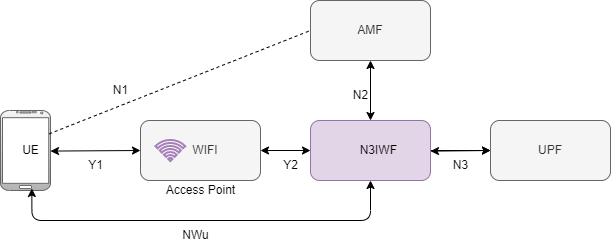
\includegraphics[width=0.8\textwidth]{figs/untrusted-non-3gpp-reg.png}
    \caption{Registration via untrusted non-\ac{3GPP} acess network}
    \label{fig:untrusted-non-3gpp-reg}
\end{figure}

\begin{figure}[htbp]
    \centering
    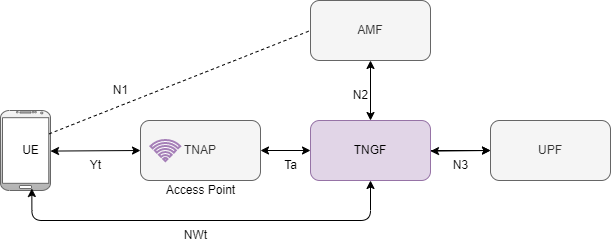
\includegraphics[width=0.8\textwidth]{figs/trusted-non-3gpp-reg.png}
    \caption{Registration via trusted non-\ac{3GPP} acess network}
    \label{fig:trusted-non-3gpp-reg}
\end{figure}

Regardless of being trusted or not, the process for an \ac{UE} to register to \ac{5GC} via a non-\ac{3GPP} Acess Network is based on a vendor-specific \ac{EAP} method called "\ac{EAP}-5G". The \ac{EAP-5G} packets utilize the "Expanded" \ac{EAP} type and the existing \ac{3GPP} Vendor-Id registered with \ac{IANA} under the \ac{SMI} Private Enterprise Code registry. The "\ac{EAP}-5G" method is used between the \ac{UE} and the \ac{N3IWF} or \ac{TNGF} and is utilized for encapsulating \ac{NAS} messages~\cite{23.502-p340}. In the case of being untrusted, if the \ac{UE} needs to be authenticated, mutual authentication is executed between the \ac{UE} and \ac{AUSF}~\cite{23.502-p325}.

\section{Wi-Fi-only Devices Integration Challenges}

As 5G advances under \ac{3GPP} and Wi-Fi evolves with Wi-Fi 6/6E and Wi-Fi 7, integrating these technologies offers significant opportunities. This convergence aims to combine the strengths of both networks for seamless, interoperable services across various use cases. However, integrating Wi-Fi-only devices into this system presents unique challenges that must be addressed.

\ac{3GPP} defines a category of devices known as \ac{N5CW} that are unable to support \ac{5G} \ac{NAS} signaling over \ac{WLAN}. These devices, while lacking direct \ac{NAS} signaling capabilities over trusted \ac{WLAN} access, can still connect to the \ac{5GC} via the \ac{TWIF} gateway function. The \ac{TWIF} handles the \ac{NAS} protocol stack and communicates with the \ac{AMF} for registration and \ac{PDU} session management on behalf of the \ac{N5CW} device over the N1 interface (as shown in Figure \ref{fig:n5cw-twap-twif}).

\begin{figure}[htbp]
    \centering
    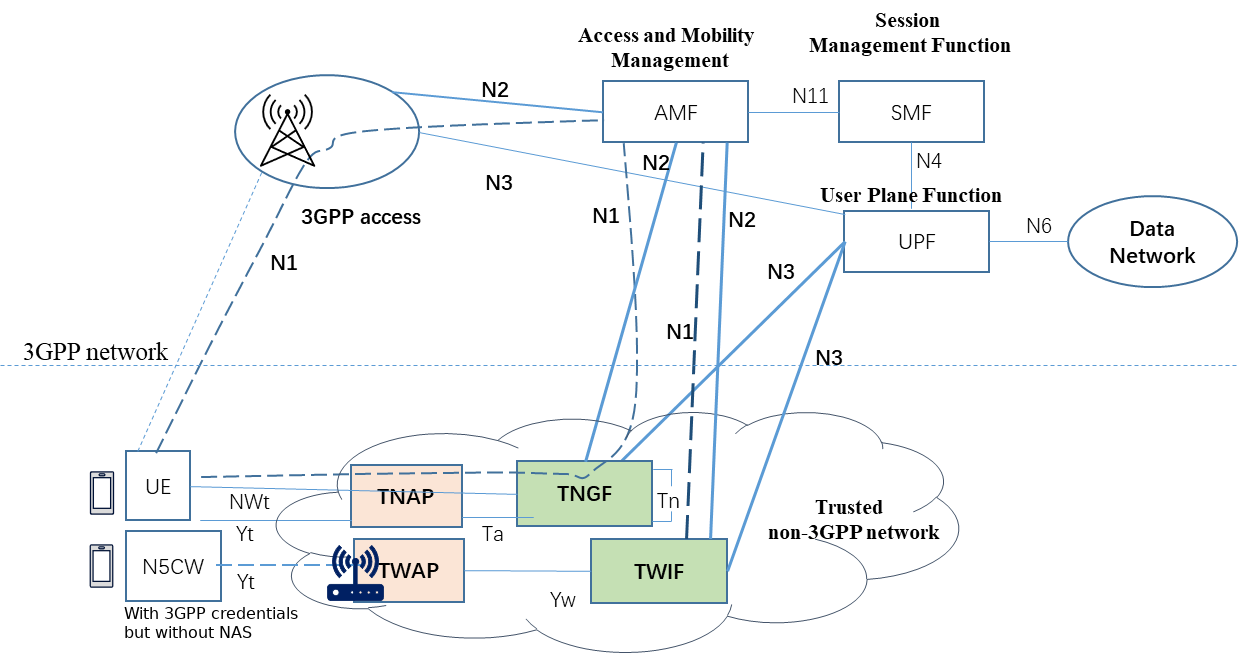
\includegraphics[width=0.8\textwidth]{figs/Authentication for devices that do, and do not support 5GC NAS over WLAN access.png}
    \caption{Authentication for devices that do, and do not, support 5GC NAS over WLAN access}
    \label{fig:n5cw-twap-twif}
\end{figure}

\ac{N5CW} devices are capable of registering with the \ac{5GC} using \ac{3GPP} credentials (or without them in certain scenarios, such as in isolated deployments or for certain IoT devices) and establishing \ac{5GC} connectivity through a trusted \ac{WLAN} access network. These \ac{3GPP} credentials are stored on the \ac{USIM}, which resides on a \ac{UICC}, a critical component for secure authentication. The \ac{USIM} provides the necessary security keys, and for devices with \ac{3GPP} access capabilities, these credentials are used for \ac{EAP}-based authentication with \ac{EAP-AKA}.

While \ac{N5CW} devices do not support \ac{NAS} signaling directly, the authentication messages are transported over the \ac{Yw} interface, with \ac{WLAN} layer-2 authentication tied to keys derived from \ac{5G} authentication procedures. The \ac{TWAP}, a particular type of a \ac{TNAP} that supports a WLAN access technology, and \ac{TWIF} are integral to enabling this process. The \ac{TWIF} is responsible for managing the \ac{NAS} protocol stack and communicating with the \ac{AMF} for registration and session management on behalf of the device, while the \ac{TWAP} is the access point that facilitates the connection to the trusted \ac{WLAN}.

The primary authentication and key agreement procedure enables mutual authentication between the device and the network, providing keying material for subsequent security procedures. The keying material generated from this authentication results in an anchor key, known as $K_{SEAF}$, which is provided by the \ac{AUSF} of the home network to the \ac{SEAF} of the serving network. This keying material can be used to derive additional keys for establishing security between the device and the trusted \ac{WLAN} access network.

The $K_{SEAF}$ is derived from an intermediate key, $K_{AUSF}$, which is established between the device and the home network during the primary authentication. This key may be securely stored in the \ac{AUSF} based on the home operator’s policy, allowing for features like Steering of Roaming or \ac{UE} Parameter Update procedures.

For Wi-Fi-only devices that lack \ac{5G} SIM credentials, the \ac{TWIF} still facilitates their integration by handling registration and session management with the \ac{5GC} on their behalf.

\subsection{Wireless and Wireline Convergence Role in Authenticating \ac{N5GC}}

Although wireline devices are not the main focus, they play a crucial role in enabling the connection of non-\ac{3GPP} devices to the \ac{5GC}. \ac{3GPP} specifies authentication procedures for both \ac{5G-RG} and \ac{FN-RG}. Unlike non-\ac{3GPP} Wi-Fi access networks, which primarily enable fixed-mobile network convergence, the \ac{5G-RG} acts as a direct bridge between the \ac{3GPP} network and the home network. The architecture for this setup is detailed in \ac{3GPP} Release 18, specifically in \ac{TS 23.316}, which describes how a \ac{5G-RG} can be configured to connect non-\ac{3GPP} devices to the \ac{3GPP} access network.~\cite{23.316}

To facilitate Wireless and Wireline Convergence in the \ac{5G} system, two new network entities are defined in \ac{TS 23.501}: the \ac{5G-RG} and \ac{FN-RG}. The \ac{5G-RG} functions as a \ac{5G} \ac{UE} and connects to the \ac{5GC} via \ac{W-5GAN} or \ac{FWA}, serving as the endpoint for \ac{N1} signaling and providing the \ac{NAS} signaling connection to the \ac{5GC} for the \ac{AUN3} devices behind it. The \ac{FN-RG}, on the other hand, connects to the \ac{5GC} via \ac{W-5GAN}, with the \ac{W-AGF} handling the registration and acting as the endpoint for \ac{N1} signaling to the \ac{5GC} on behalf of the \ac{FN-RG}. Additionally, a \ac{5G}-capable \ac{UE} can connect to the \ac{5GC} through an RG using \ac{W-5GAN} or \ac{NG-RAN}, supporting both trusted and untrusted non-\ac{3GPP} access.

As specified in \ac{TS 33.501} clause 7B.7.1, an \ac{AUN3} device behind a \ac{5G-RG}, as defined in \ac{TS 23.316}, must be registered to the \ac{5GC} by the \ac{5G-RG} and authenticated by the \ac{5GC} using \ac{EAP-AKA'}. The \ac{AUN3} device is required to send an \ac{EAP} Response/Identity containing its \ac{NAI} in the format \texttt{username@realm}. If the \ac{AUN3} device supports \ac{SUPI} privacy, it must include a \ac{SUCI} in the \ac{EAP} Response/Identity.

If the \ac{AUN3} device provides an \ac{NAI}-based \ac{SUPI}, the \ac{5G-RG} must generate a \ac{SUCI} using the null-scheme based on the \ac{NAI}-based \ac{SUPI}. The \ac{5G-RG} then sends a \ac{NAS} Registration Request message to the \ac{AMF}, including the \ac{SUCI} of the \ac{AUN3} device and an \ac{AUN3} device indicator.

When dealing with devices behind gateways, 3GPP provides a scenario regarding the authentication procedure, using EAP-TLS as an example~\cite{TS 33.501 Annex O}, for \ac{N5GC} devices behind \acp{RG} in private networks or in isolated deployment scenarios (i.e., roaming is not considered). These devices lack \ac{SIM} cards and traditional \ac{3GPP} credentials and do not support \ac{NAS} signaling or the \ac{5G} key hierarchy derivation but are designed to access the converged \ac{5G} Core Network (\ac{5GCN}) through non-\ac{3GPP} access methods.

Let't go over the key details about this scenario:

\begin{enumerate}
    \item{
        Network Infrastructure
        \begin{itemize}
            \item{
                \ac{N5GC} devices connect to access points (\acp{AP}) that are part of wireline network infrastructures.
            }
            \item{
                The term "wireline" does not refer to the device itself, but to the network infrastructure which involves physical cables (e.g., fiber optic, coaxial, or twisted pair) rather than the devices themselves.
            }
            \item{
                These devices are considered to "exist in wireline networks" because their data transmission often involves wireline components, despite the fact that their immediate connection could wireless via Wi-Fi, such as a smartphone or IoT device in a home network.
            }
        \end{itemize}
    }
    \item{
        Authentication
        \begin{itemize}
            \item{
                Unlike traditional \ac{5G} \ac{UE}s, \ac{N5GC} devices do not rely exclusively on \ac{EAP-AKA'} for authentication.
            }
            \item{
                They can use other \ac{EAP} methods, providing flexibility for integrating legacy IoT devices, smart home appliances, or other non-\ac{3GPP} Wi-Fi-capable equipment.
            }
            \item{
                These devices do not require \ac{USIM}-based credentials, allowing for authentication without a physical \ac{SIM} card.
            }
        \end{itemize}
    }
    \item{
        Authentication
        \begin{itemize}
            \item{
                Unlike traditional \ac{5G} \ac{UE}s, \ac{N5GC} devices do not rely exclusively on \ac{EAP-AKA'} for authentication.
            }
            \item{
                They can use other \ac{EAP} methods, providing flexibility for integrating legacy IoT devices, smart home appliances, or other non-\ac{3GPP} Wi-Fi-capable equipment.
            }
            \item{
                These devices do not require \ac{USIM}-based credentials, allowing for authentication without a physical \ac{SIM} card.
            }
        \end{itemize}
    }
\end{enumerate}

The \ac{3GPP} procedure for \ac{N5GC} device authentication employs \ac{EAP-TLS} with specific characteristics. During the registration process (as seen in Figure \ref{fig:n5gc-eap-tls}), the \ac{W-AGF} acts on behalf of the \ac{N5GC} device and creates the registration request. \ac{5G} parameters such as \ac{ngKSI} and \ac{ABBA} are not sent to the \ac{N5GC} device. If these parameters are received from the \ac{AMF}, the \ac{W-AGF} ignores them. Additionally, neither the \ac{N5GC} device nor the \ac{AUSF} derives any \ac{5G}-related keys after \ac{EAP} authentication.

\begin{figure}[htbp]
    \centering
    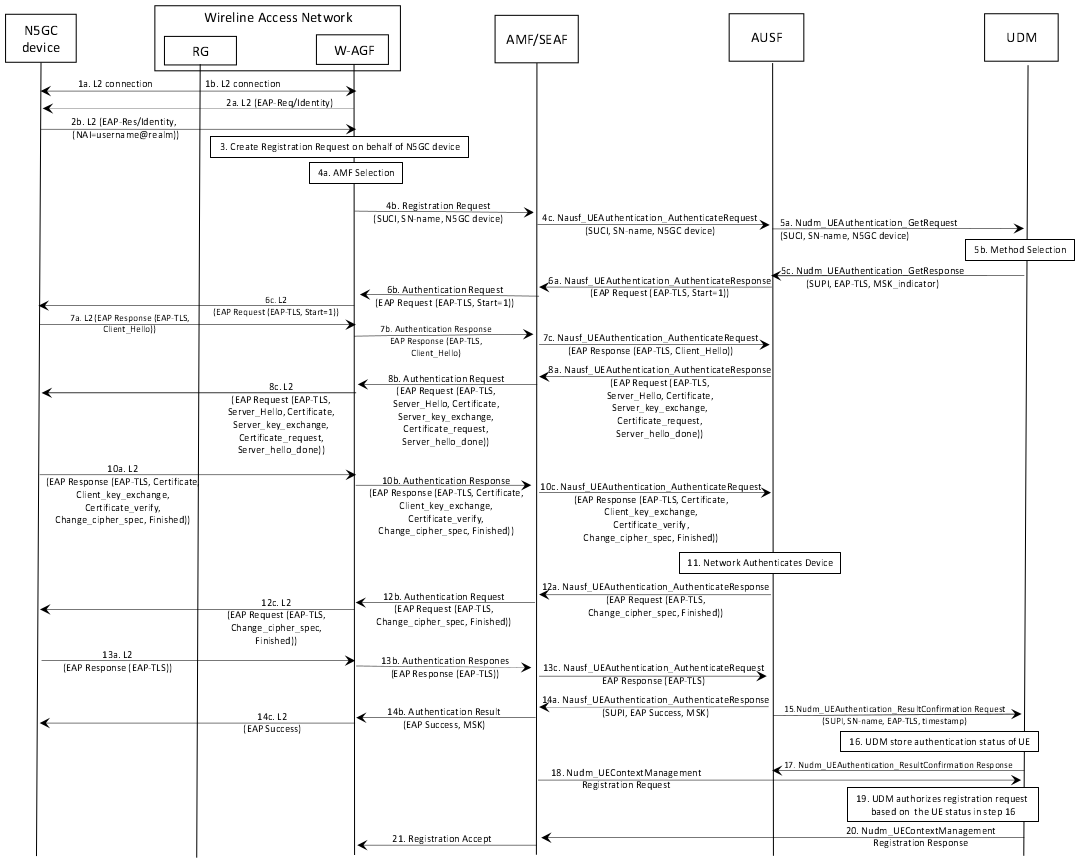
\includegraphics[width=0.8\textwidth]{figs/Registration and authentication of a non-5G capable device to the 5GC.png}
    \caption{Registration and authentication of a non-5G capable device to the 5GC}
    \label{fig:n5gc-eap-tls}
\end{figure}

While the procedure specifies \ac{EAP-TLS}, other \ac{EAP} methods can also be supported. The link between the \ac{N5GC} device and the \ac{RG}, as well as the link between the \ac{RG} and the \ac{W-AGF}, can utilize any \ac{L2} data link that supports \ac{EAP} encapsulation.

TS 23.316 also describes support for specific devices, including \ac{AUN3}, \ac{NAUN3} and \ac{N5GC}. 

From this specification, particularly at clause 4.10a, we learn some important details regarding identity construction and mapping during the registration process. The \ac{N5GC} device initiates a connection by relying on the \ac{CRG} operating in L2 bridge mode, which forwards any L2 frames to the \ac{W-AGF}. The \ac{802.1x} authentication can be triggered either when the \ac{N5GC} device sends an \ac{EAPOL}-Start frame or when the \ac{W-AGF} detects an unknown \ac{MAC} address. The \ac{CRG}'s configuration in bridge mode and the triggering mechanism for the \ac{W-AGF}'s handling of \ac{N5GC} devices are specified in the CableLabs \ac{WR-TR-5WWC-ARCH} standard. During this process, the \ac{N5GC} device sends an \ac{EAP}-Response/Identity message, which includes its \ac{NAI} formatted as \texttt{username@realm}.

Upon receiving the \ac{NAI} through \ac{EAP}-Identity, the \ac{W-AGF} constructs a \ac{NAS} Registration Request message on behalf of the \ac{N5GC} device, marking the device as non-\ac{5G} capable. This request includes a \ac{SUCI}, which the \ac{W-AGF} generates from the received \ac{NAI}, as defined in \ac{TS} 33.501. The \ac{W-AGF} sends this \ac{NAS} Registration Request to the \ac{AMF} for further processing.

Subsequently, the \ac{EAP}-based authentication procedure, as outlined in \ac{TS} 33.501, is executed between the \ac{N5GC} device and the \ac{AUSF}. If the authentication succeeds, the \ac{AUSF} shares security-related details, including the \ac{SUPI} corresponding to the \ac{NAI}, with the \ac{AMF}. Each \ac{N5GC} device is uniquely registered to the \ac{5GC} using its \ac{SUPI} after successful authentication.

Finally, the \ac{AMF} performs the required registration procedures in accordance with \ac{TS} 23.502. When the \ac{W-AGF} provides the \ac{PEI} for the \ac{N5GC} device, it encodes the device's \ac{MAC} address. Depending on the operator's policy, the \ac{MAC} address can be formatted using the \ac{IEEE} \ac{EUI}-64 standard. This ensures proper identification and registration of the \ac{N5GC} device within the \ac{5GC}.

Also in TS 23.216, clause 4.10b defines support for \ac{NAUN3} devices behind \ac{5G-RG}. \ac{NAUN3} devices, which are not \ac{3GPP}-capable, cannot be authenticated by the \ac{5GC}. These devices do not natively support \ac{3GPP} protocols and therefore rely on alternative authentication methods. For example, \ac{NAUN3} devices can be locally authenticated by the \ac{5G-RG} using mechanisms such as a pre-shared secret. This pre-shared secret could include something like a WiFi password, as it represents a locally managed credential used to establish trust between the device and the \ac{5G-RG}.

Despite their limitations, \ac{NAUN3} devices can still benefit from differentiated services, such as \ac{QoS} or network slicing, as defined in this clause. The concept of "Connectivity Group IDs" is introduced, where each \ac{Connectivity Group ID} corresponds to a distinct physical or virtual port on the \ac{5G-RG}. Examples of such ports include physical Ethernet ports, separate \ac{WLAN} \ac{SSID}s, or a \ac{VLAN}. Devices that connect through a particular logical port are grouped under the same \ac{Connectivity Group ID}. The configuration of these ports on the \ac{5G-RG} is considered out of scope for this specification.

\begin{figure}[htbp]
    \centering
    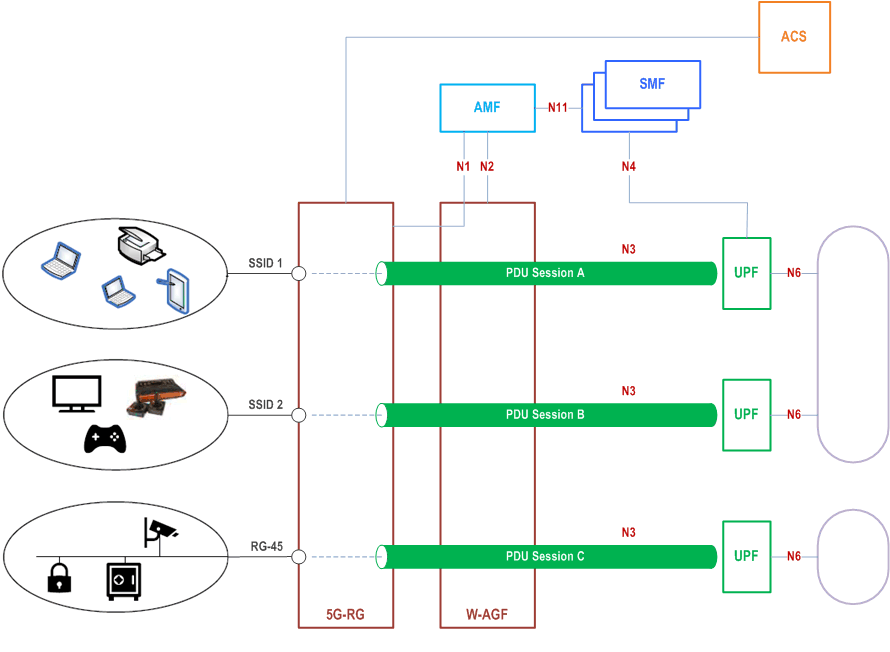
\includegraphics[width=0.8\textwidth]{figs/Example scenario for NAUN3 devices behind 5G-RG based on connectivity groups.png}
    \caption{Example scenario for NAUN3 devices behind 5G-RG based on connectivity groups}
    \label{fig:naun3-bhd-5grg}
\end{figure}

Each \ac{Connectivity Group ID} is linked to a unique \ac{PDU Session} (as shown in Figure \ref{fig:naun3-bhd-5grg}) established by the \ac{5G-RG} following procedures defined in clause 7. The \ac{5G-RG} is pre-configured with virtual port information, such as \ac{VLAN}s and \ac{SSID}s, using standards like \ac{TR}-69, \ac{TR}-360, and \ac{TR}-181. Additionally, \ac{URSP} rules can be delivered to the \ac{5G-RG} to map each \ac{Connectivity Group ID} to the parameters of the associated \ac{PDU Session}, such as the \ac{DNN} and \ac{S-NSSAI}. Note that the mapping between virtual ports and parameters like \ac{DNN} or \ac{S-NSSAI} can also be configured using \ac{TR}-69 or \ac{TR}-181. However, the specification does not cover how \ac{NAUN3} devices are configured to use a particular \ac{SSID} or connect to a specific Ethernet port on the \ac{5G-RG}.

Further differentiation in charging and \ac{QoS} is achievable through \ac{PCC} rules that define different service flows tied to dedicated \ac{PDU Sessions} for \ac{NAUN3} devices. Additionally, the isolation of devices belonging to a specific \ac{Connectivity Group ID} can be implemented through a specific network slice, i.e., by associating them with a distinct \ac{S-NSSAI}.

%\subsection{Wireless Broadband Alliance (WBA) recommendations}

%\subsection{WBA Private 5G and Wi-Fi Convergence}

\section{Current Solutions and Proposals}'